\documentclass[letter, 11pt]{article}
\usepackage[margin=1in,centering]{geometry}
\usepackage{amsmath}

\usepackage{tikz}
\usepgflibrary{arrows}
\usetikzlibrary{calc,intersections,through,backgrounds}

\begin{document}
\pagestyle{empty}

\section*{Problem Statement}
The pivot point of a simple pendulum having a natural period of 1.00 second is
moved laterally in a sinusoidal motion with an amplitude 1.00 cm and period
1.10 seconds. With what amplitude should the pendulum bob swing after a steady
motion is attained?

\section*{Solution}
The first step in the solution process is to obtain the equation of motion. To
this end, I introduce a few symbols to represent physical quantities: $m$, $l$,
$g$, $F_g$, $F_r$, being the mass of the pendulum, the length from the pendulum
pivot to the mass center, the gravitational constant, the gravitational force
acting on the mass, and the force acting on the mass from the rod,
respectively. Without loss of generality, I assume a simple point mass pendulum
with a massless rod.

\begin{figure}[!hbp]
  \centering
  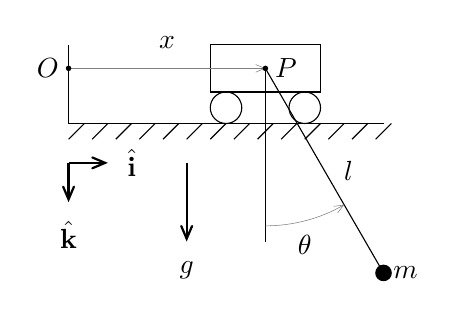
\begin{tikzpicture}[>=angle 45, auto]

    % First draw the ground
    \draw (0, 1) -- (0,0) -- (4,0);
    \foreach \x in {0, .3, ..., 4}
      \draw (\x, -.2) -- (\x+0.2, 0);

    % Next, draw the cart
    \draw (2.0, 0.2) circle (0.2cm);
    \draw (3.0, 0.2) circle (0.2cm);
    \draw (1.8, .4) rectangle (3.2, 1.0);

    % Define a few points
    \coordinate [label=left:{$O$}] (O) at (0.0, .7);
    \coordinate [label=right:{$P$}] (P) at (2.5, .7);
    \coordinate [label=right:{$m$}] (M) at (4.0, -1.898);
    \coordinate (A0) at (2.5, -1.3);
    \coordinate (A1) at (3.5, -1.032);

    \draw[very thin] (P) -- (2.5, -1.5);

    \draw[->, very thin, gray] (O) -- (P);
    \foreach \point in  {O, P}
      \fill [black] (\point) circle(1pt);
    \node [label=above:$x$] (X) at ($ (O)!.5!(P) $) {};

    \fill [black] (M) circle(3pt);
    \node [label=right:$l$] (L) at ($ (P)!.5!(M) $) {};
    \draw (P) -- (M);

    \draw[->, very thin, gray] (A0) arc (-90:-60:2.0);
    \node [label=below:$\theta$] (T) at ($ (A0)!.5!(A1) $) {};


    \coordinate (CO) at (0.0, -0.5);
    \coordinate (X) at (0.5, -0.5);
    \coordinate (Y) at (0.0, -1.0);
    \node [label=right:$\hat{\mathbf{i}}$] (I) at (X) {};
    \node [label=below:$\hat{\mathbf{k}}$] (J) at (Y) {};
    \draw[->, thick] (CO) -- (X);
    \draw[->, thick] (CO) -- (Y);
    \draw[->, thick] ($ (X) + (1.0, 0.) $) -- ++(0, -1.0);
    \node [label=below:$g$] (G) at (1.5, -1.5) {};
  \end{tikzpicture}
  \caption{Pendulum with horizontally translating pivot. $\hat{\mathbf{j}} = \hat{\mathbf{k}} \times \hat{\mathbf{i}}$ points out of
  the page.}
  \label{fig1}
\end{figure}

%Let $O$ be a point fixed in an inertial reference frame $N$.  The position from $O$ to $P$ is
%\[
%\mathbf{r}^{OP} = 0.01\sin\left(\frac{2\pi}{1.1}t\right) \hat{\mathbf{i}}
%\]
%and the acceleration of $P$ relative to the inertial frame $N$ is
%\[
%\mathbf{a}^{P}=
%-0.01\left(\frac{2\pi}{1.1}\right)^2\sin\left(\frac{2\pi}{1.1}t\right)
%\hat{\mathbf{i}}
%\]
The velocity and acceleration of the pendulum mass relative to an inertial
frame are
\begin{align*}
\mathbf{v} &= \dot{x}\hat{\mathbf{i}} + \dot{\theta} \hat{\mathbf{j}} \times \left(l
\sin \theta \hat{\mathbf{i}} + l \cos \theta \hat{\mathbf{k}}\right)\\
&= \left(\dot{x} + l \dot{\theta} \cos \theta \right)\hat{\mathbf{i}} +
\left(-l \dot{\theta} \sin \theta \right) \hat{\mathbf{k}} \\
\mathbf{a} &= (\ddot{x} + l \ddot{\theta} \cos \theta - l \dot{\theta}^2 \sin
\theta) \hat{\mathbf{i}} + (-l \ddot{\theta} \sin \theta - l \dot{\theta}^2
\cos\theta)\hat{\mathbf{k}}
\end{align*}
Two forces act on the mass; the gravitational force $\mathbf{F}_g$ and the force
of the rod $\mathbf{F}_r$:
\[
\mathbf{F}_g = mg\hat{\mathbf{k}} \qquad \mathbf{F}_r = - F \sin \theta
\hat{\mathbf{i}} - F \cos \theta \hat{\mathbf{k}}
\]
where $F$ is a function of time.  Newton's 2nd law yields:
\[
mg\hat{\mathbf{k}} - F \sin \theta \hat{\mathbf{i}} - F \cos \theta
\hat{\mathbf{k}} = m (\ddot{x} + l \ddot{\theta} \cos \theta - l \dot{\theta}^2 \sin
\theta) \hat{\mathbf{i}} + m (-l \ddot{\theta} \sin \theta - l \dot{\theta}^2
\cos\theta)\hat{\mathbf{k}}
\]
Dotting this equation with $\cos\theta\hat{\mathbf{i}} - \sin \theta \hat{\mathbf{k}}$, dividing
through by $m$ and rearranging, yields:
\[
\ddot{\theta} + \frac{g}{l} \sin \theta =
0.01\left(\frac{2\pi}{1.1}\right)^2\sin\left(\frac{2\pi}{1.1}t\right) \cos
\theta
\]
Notice how dotting the Newton's equation into the direction perpendicular to
the rod is a convenient way to eliminate the constraint force
$\mathbf{F}_r$. Linearizing about the downwards position $\theta = 0$, we have
$\sin \theta \approx \theta$ and $\cos \theta \approx 1$, which yields the
following second order linear differential equation:
\[
\ddot{\theta} + \frac{g}{l} \theta =
0.01\left(\frac{2\pi}{1.1}\right)^2\sin\left(\frac{2\pi}{1.1}t\right)
\]
Defining $\omega_n^2 = \frac{g}{l}$ and $f_0 =
0.01\left(\frac{2\pi}{1.1}\right)^2$, and $\omega = \frac{2\pi}{1.1}$, we can
rewrite the equation of motion as
\[
\ddot{\theta} + \omega_n^2 \theta = f_0 \sin \omega t
\]
Assuming a particular solution of the form $\theta_p(t) =
\Theta\sin\omega t$, differentiating twice with respect
to time, and substituting into the equation of motion yields:
\[
(-\omega^2 + \omega_n^2)\Theta \sin\left(\omega t \right) = f_0 \sin
\omega t
\]
which implies that the amplitude of swing of the pendulum bob after steady
motion is attained is:
\begin{align*}
  \Theta &= \frac{f_0}{\omega_n^2 - \omega^2} \\
         &= \frac{0.01\left(\frac{2\pi}{1.1}\right)^2}{(2\pi)^2 -
         (\frac{2\pi}{1.1})^2} \\
         &= 0.047619 \quad \text{rad}\\
         &= 2.7284 \quad \text{deg}
\end{align*}
Where we made use of the fact that the natural frequency is related to the
natural period of oscillation by $\omega_n = 2\pi / T = 2\pi$ rad/s.

Note that this solution does not depend in any way on the physical parameters I
introduced to show the derivation of the equation of motion, it only depends on
the natural frequency of the pendulum, and the magnitude and frequency of the
horizontal displacement. This solution is only valid for small angles, and
assumes that friction is negligible.

\end{document}
